\chapter{Results}\label{chap3}
\thispagestyle{plain}

As mentioned in Section \ref{chap2}, three machine learning algorithm have been used to train models based on ice thickness observations and predict ice thicknesses. The same procedure has been applied to all the algorithm used in order to be able to compare the results between the different models. 
All the algorithm have been trained and tested using the data available in the GlaThiDa data-set in the alpine region. Only glaciers present in the GlaThiDa database belonging to Region 11 of the RGI (Central Europe) have been used in the following analysis. This corresponds to glaciers present in the alps. 
After training each algorithm the resulting model has been used to predict the ice volume of all the glaciers in the alps. This is useful to compare the results of these model to those computed by Farinotti et al. in \citet{Farinotti2019}.

\section{Results from Linear Regression}\label{linear}
The first model to be analyzed is the one obtained from training the linear regression algorithm. In order to asses the how well a machine learning model makes predictions a sub-sample of the data-set is usually left out from the training process (see Section \ref{training}). With the left out data the score from Eq. \ref{eq:score} is computed by letting the model predict the values not used for training. This is done to make sure the model is not over-fitted. Complex machine learning algorithm in fact might be very good at predicting data inside the training sample but might perform much worse on data outside this sample (over-fitting). 
This is usually not the case with linear regression, hence in principle there is no need to only use a sub-sample of the data to train the model. The $R^2$ coefficient could be computed using the whole data-set to train the model. Following however the linear regression algorithm has been trained using the same procedure used for the other algorithms to be able to better compare the models with each other and try to find similarities and differences.     

\subsection{Score and volume spread}\label{lr-score}

\begin{figure}[!tp]
	\centering		  
	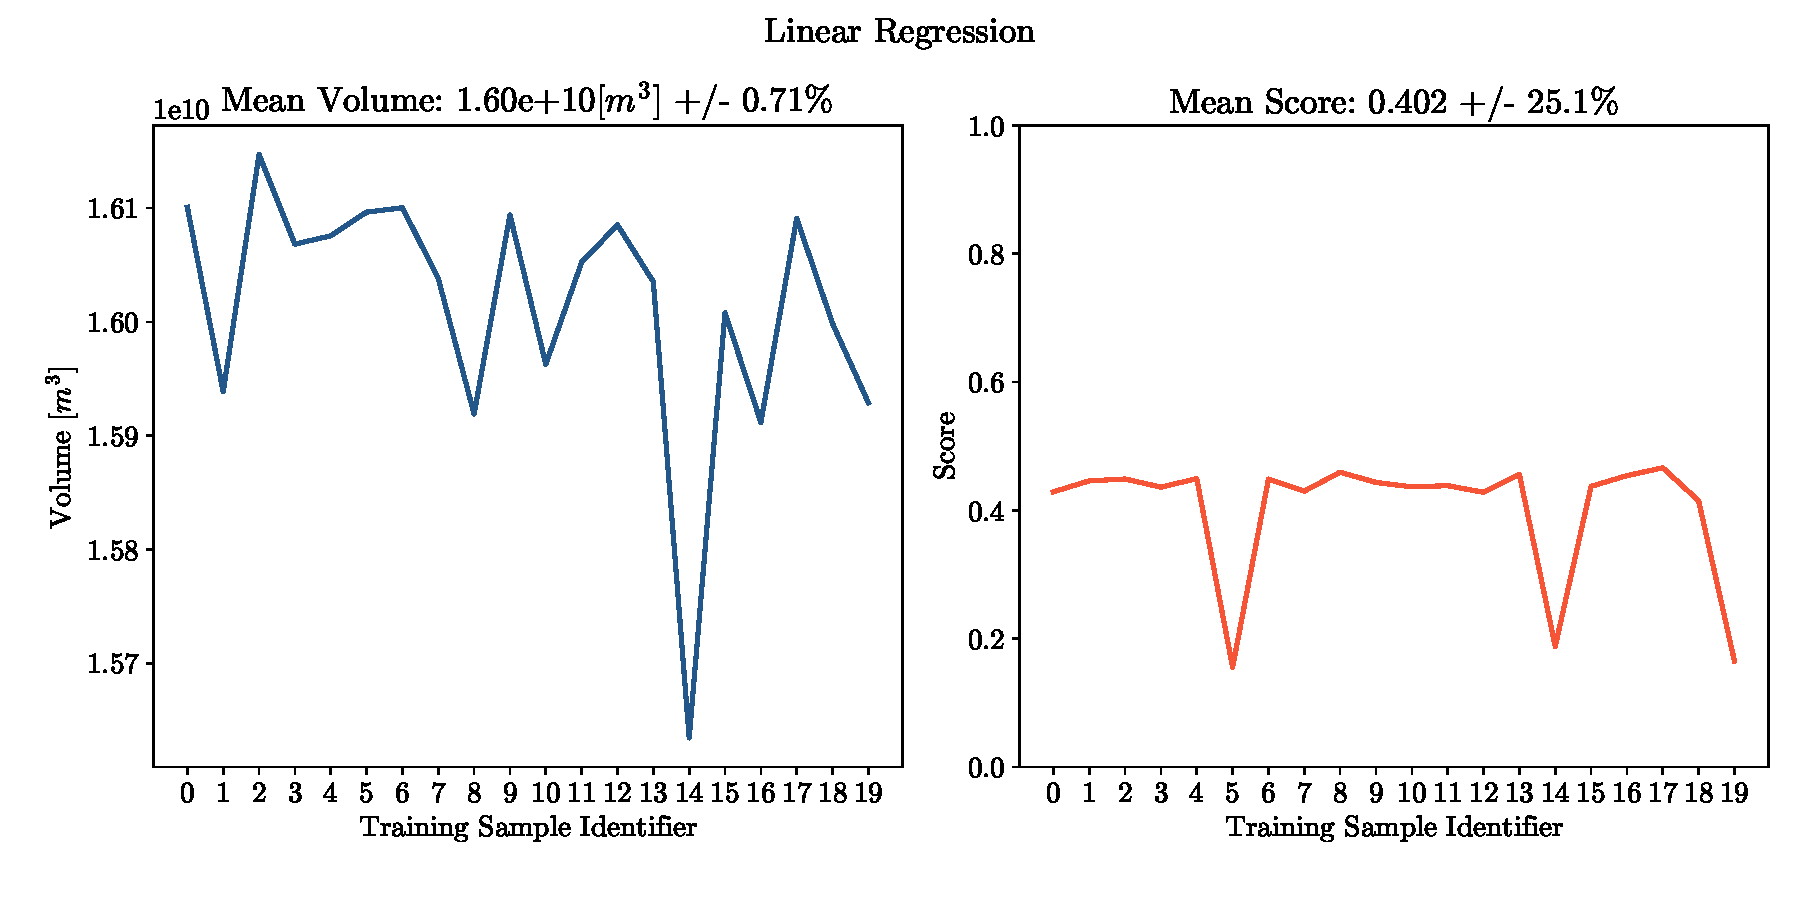
\includegraphics[width=1.\textwidth]{figures/LR_score.pdf}
	\caption{Linear Regression: Volume and score values of the model after training it with 20 different sub-sample of data. On the x-axis each number identifies a different sample of data. On the left the total volume of the alpine glaciers present in the GlaThiDa. On the right the $R^2$ coefficient for values left out of the training sample.}
	\label{fig:lr-score}
\end{figure}

Figure \ref{fig:lr-score} shows the volume and score change  for 20 different sub-samples used for training the linear regression algorithm. Each number on the x-axis represents a different sample used for training: of all the alpine glaciers observations in the GlaThiDa, 75\% of them have been used for  training the model and the resulting 25\% to compute the score. 

The volume show in the right side of Figure \ref{fig:lr-score} has been computed on the full sample of glaciers but each time using the different model derived from training it with each sub-sample. The mean volume for the 20 different sub-samples is $1.60\times 10^{10}$ $m^3$ with a relative standard deviation of 0.74\%. Sample 14 clearly predicts the lowest of all volumes.

It is worth nothing that the model predicts ice thicknesses below zero for certain points. These have however been rounded to zero as a thickness below zero makes no physical sense.

The average score is 0.402 with a high 25.1\% relative standard deviation. Clearly this is due to the score dropping for sub-samples 5, 14 and 19. For most sub-samples the score is in fact above 0.4 but for those three it drops even below 0.2. Sub-sample 14 then leads to the lowest volume and a low score compared to the average. 


\subsection{Features Importance}  

\begin{figure}[!tp]
	\centering		  
	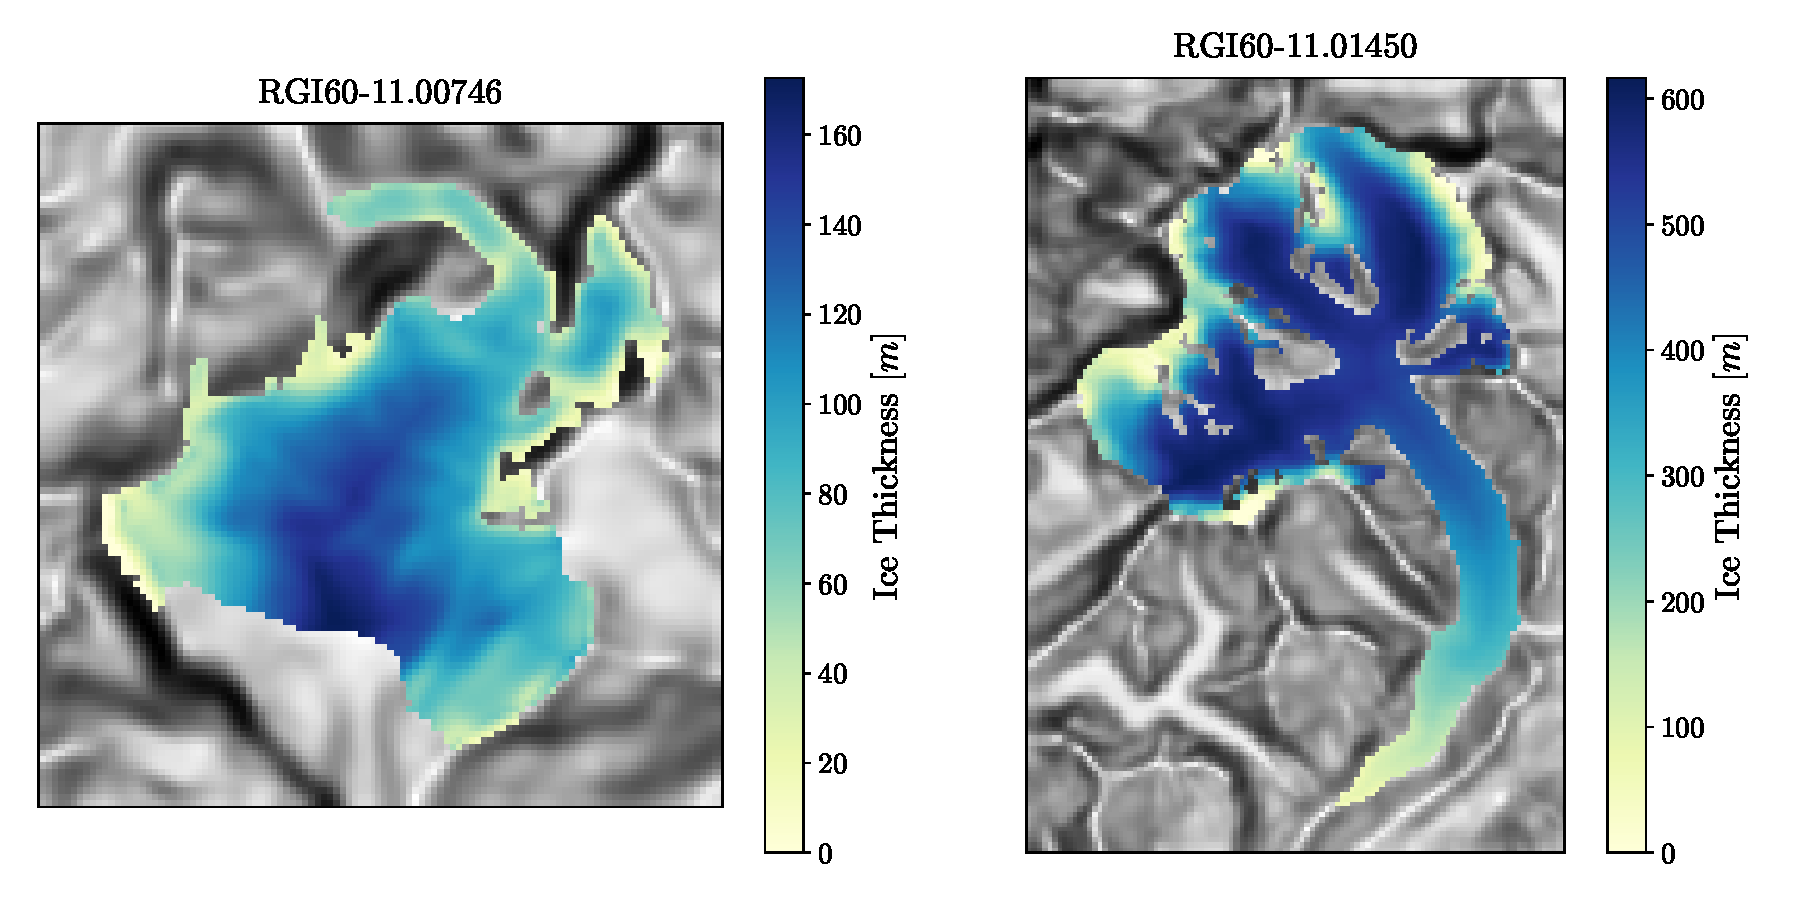
\includegraphics[width=1.\textwidth]{figures/LR_thick_map.pdf}
	\caption{Linear Regression: Ice thickness distribution for two glaciers on top of the terrain slope angle. On the left one of the glaciers used for training the model. On the one of the glaciers outside those used for training the model.}
	\label{fig:lr-map}
\end{figure}

\begin{table}
	\centering
	\caption{Linear Regressions: Coefficients for the linear regression model: higher absolute values mean that the feature have a higher influence on the model predictions}
	\begin{tabular}{|c|c|c|c|}
		\hline 
		Slope&Mass Balance&Distance From Border&Altitude \\
		\hline
		-19.7&12.7&7.7&-6.6 \\
		\hline
	\end{tabular}
\label{tb:lr-coef}
\end{table}

It is interesting to look into which of the variables used to train the model influence the outcome of the prediction the most.
A very easy way to do so for a linear regression model is just to analyze the weights $\bm{\beta}$ (see Eq. \ref{eq:linear}) which the model assigned to each feature in order to make predictions. These are shown in Table \ref{tb:lr-coef}.
The higher the absolute values of the coefficients, the more the variable will influence the outcome of the model. In this case the slope is the feature which is more relevant to the outcome of the model followed by the linear mass balance. In particular the slope is influences the prediction almost 3 times more than the altitude and over 2.5 times more than the distance from the border. This means that a doubling of the slope angle of the glacier surface will result in an ice thickness change 3 times larger than the change that would occur in a doubling of the altitude. \todo{Talk about sign of slope angle; reference equation from book}


\begin{itemize}
	\item[(1)] Score plots
	\item[(2)] Volume spread plots
	\item[(3)] Glacier maps
	\item[(4)] Features importance
	\item[(5)] Volume for the whole alps
\end{itemize}

\section{SVM}\label{svm}
Results from the SVM
\begin{itemize}
	\item[(1)] Score plots
	\item[(2)] Volume spread plots
	\item[(3)] Glacier maps
	\item[(4)] Features importance
	\item[(5)] Volume for the whole alps
\end{itemize}

\section{Random forest}\label{rfr}
Results from the Random Forest
\begin{itemize}
	\item[(1)] Score plots
	\item[(2)] Volume spread plots
	\item[(3)] Glacier maps
	\item[(4)] Features importance
	\item[(5)] Volume for the whole alps
\end{itemize}


% ==== SECTION 1 ===============================================================
%\section{Some Important Things to Know}\label{3sec:1}
%
%It is important to differentiate between \emph{facts} and \emph{interpretations}
%and between \emph{your contributions} and \emph{those of others}! Facts and
%your contributions are part of this chapter. Interpretations and contributions
%of others should be rather part of the chapter Discussion.
%
%
%\subsection{Experimental Parts in the Chapter Results}
%Experimental details should only appear in the chapter Results to the
%extent necessary to ensure comprehension. Painstaking descriptions of
%instruments, analysis procedures, field conditions, etc., should be part of the
%chapter Methodology. However, absolutely necessary is information that shows
%the \emph{reliability} of the findings and the \emph{robustness} of an
%innovation (e.g., a new analysis technique).
%
%
%\subsection{Numerical Results or so-called Data}
%Results are more than simply numbers! They are tiny but unique
%\emph{messages}. Data should not only be made ``visible'' (e.g., in
%figures, such as in Fig.~\ref{fig:1}) but should also be made
%\emph{articulate}.
%
%
%\subsection{Order of Presentation}
%Use chapters and (sub)sections to separate, e.g., various topics,
%questions, and problems, or to separate measurements from calculations. 
%Arrange information in a consistent way, e.g., from simple to complex, from
%small to large (or vice versa in terms of scales: e.g., from
%synoptic-scale to micro-scale), from \emph{most important} (central) to
%\emph{least important} (peripheral). Arrange the material in order to maximize
%impact rather than sticking to a strict chronological order. Try to tell a story
%that consists of a beginning, followed by a gradual unfolding, and a
%``happy end''.
%
%
%\subsection{Cross-References}
%You can always refer to other parts of your thesis like in the following
%example: See chapter \ref{chap2} or section \ref{1sec:3} or
%Fig.~\ref{fig:1} or Table~\ref{tab:1} or equation~(\ref{2equ:1}).
%
%
%\section{Figure}\label{3sec:2}
%Figure \ref{fig:1} shows an example for an EPS figure with two panels. The
%topography of the Wipp Valley and Inn Valley is shown in Fig.~\ref{fig:1a}.
%Figure~\ref{fig:1b} shows the time series of potential temperature at two
%stations. In order to refer to a certain range of figure panels write, e.g.,
%Fig.~\ref{fig:1a}--\subref{fig:1b}.
%
%
%\begin{figure}[!tp]
%\centering
%\figuretopcapfalse
%\subfigure[][]{
%  \label{fig:1a}  
%  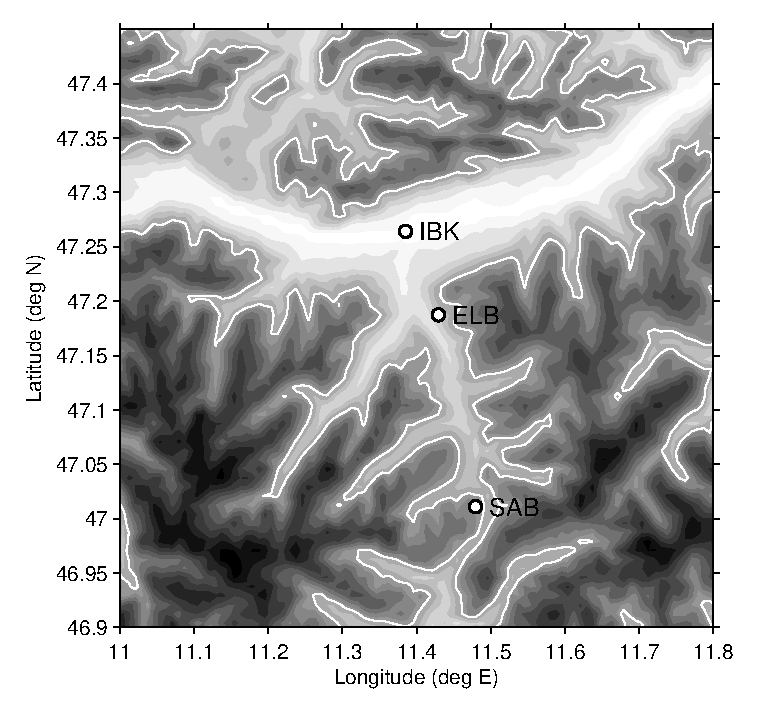
\includegraphics[width=0.48\textwidth]{figure_topo.eps}
%}
%\subfigure[][]{
%  \label{fig:1b}
%  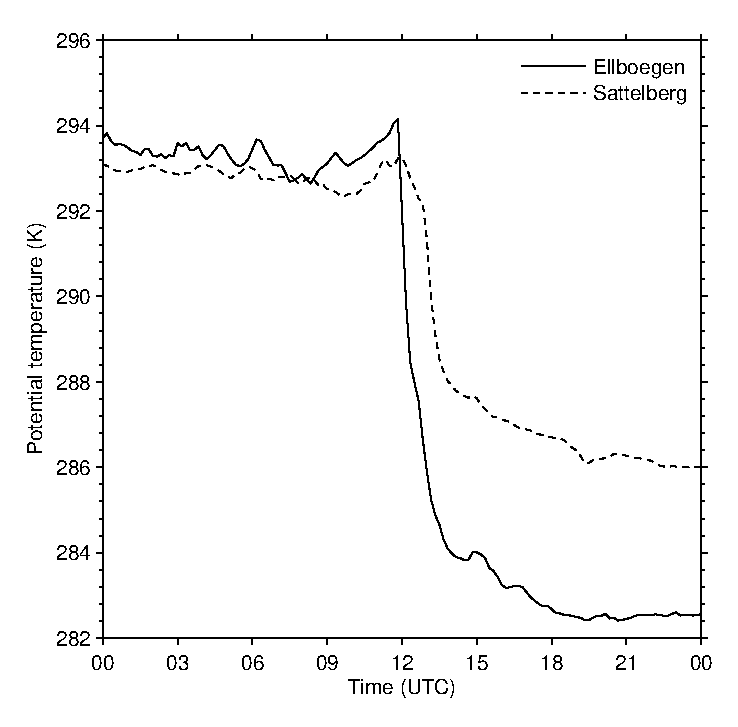
\includegraphics[width=0.47\textwidth]{figure_theta.eps}
%}
%\caption{(\subref{fig:1a}) Topographic map of the target area: Gray shaded
%elevations contours with increments of 200~m starting at 400~m~MSL and a white
%elevation contour line at 1600~m MSL. (\subref{fig:1b}) Time series of potential
%temperature (K) at Ellboegen (solid line) and Sattelberg (dashed line) from 00
%UTC 06 November to 00 UTC 07 November 1999. Labels in (\subref{fig:1a}) mark the
%location of Innsbruck (IBK), Ellboegen (ELB), and Sattelberg
%(SAB).}\label{fig:1}
%\end{figure}
%
%
This template uses the \texttt{subfigure} environment with the option
\texttt{FIGTOPCAP} to place the subfigure labels (\subref{fig:1a}) and
(\subref{fig:1b}) at the top of the figure. However, since we want to have the
caption at the bottom of figure, use \verb|\figuretopcapfalse|
before the first \verb|\subfigure| command within the \texttt{figure}
environment, otherwise the figure number produced by \verb|\ref| is wrong.
%
%
%\section{Table}
%Table \ref{tab:1} is an example for a table that consists of several
%rows and columns. Here, the \texttt{tabular} environment is used inside the
%\texttt{table} environment.
%
%
%\begin{table}[!htb]
%\centering
%\begin{footnotesize}
%\renewcommand{\tabcolsep}{4pt}
%\begin{tabular}{l p{3.5cm} l l l}
%\hline
%\hline
%Parameter & Code & Description & Units & Code\\
%\hline
%$g$ & \verb|$g$| & acceleration due to gravity&
%  m~s$^{-2}$ & \verb|m~s$^{-2}$| \\
%$T_d$ & \verb|$T_d$| & dew point temperature & $^{\circ}$C & 
%  \verb|$^{\circ}$C| \\
%$\mathbf{v} \cdot \nabla T$ & \verb|$\mathbf{v} \cdot| \verb| \nabla T$| &
%  temperature advection & K~s$^{-1}$ & \verb|K~s$^{-1}$| \\
%$\vec{v} \cdot \nabla T$ & \verb|$\vec{v} \cdot| \verb| \nabla T$| & 
%  temperature advection & K~s$^{-1}$ & \verb|K~s$^{-1}$| \\
%$\frac{\partial p}{\partial t}$ & \verb|$\frac{\partial p}|
%  \verb| {\partial t}$| & local pressure tendency & Pa~s$^{-1}$ &
%  \verb|Pa~s$^{-1}$| \\
%$p_0 \cos (kx - \omega t)$ & \verb|$p_0 \cos (kx| \verb| - \omega t)$| &
% wave expression & Pa & Pa \\
%\hline
%\end{tabular}
%\end{footnotesize}
%\caption{Some meteorological and mathematical parameters and expressions.}
%\label{tab:1}
%\end{table}
%
%
%\section{Figure and Table Captions}
%
%Figure and table captions \emph{must} contain all necessary information to
%understand the \emph{content} of the figure and table, without the need of
%additional text. Only in case of very complicated figures or tables, the caption
%may end with a remark such as ``See text for further explanation''. The
%\emph{interpretation} of the table or figure is not part of the caption, but
%should be given in the main text. In order to avoid repetitions, the phrase
%``As in Fig. xx, but for \dots'' is often used. Necessary information provided
%in the caption is a description of
%\begin{itemize}
%\item shown parameters together with units,
%\item date and time,
%\item contour intervals,
%\item location,
%\item line styles and markers,
%\item and others.
%\end{itemize}
%A list of figures and a list of tables at the beginning of the thesis (before
%chapter 1) is optional.
%
%
%
%\section{Title}
%
%The title of your science thesis should be kept as short as possible. It should
%represent an extremely compact summary of the thesis. The title should provide a
%clear and complete description of the topic and should contain many keywords
%(``what?'', ``how?'' and possibly ``why?''). The main title should not contain
%more than 10 words. An optional subtitle may be used if necessary (all together
%not more than 25 words). Important words and terms should be placed at the
%beginning of the title. Avoid unspecific expressions such as
%\begin{itemize}
%\item[] Investigation of ...
%\item[] Experiments on ...
%\item[] Results of ...
%\item[] Attempts to ...
%\end{itemize}
%Rather use expressions such as
%\begin{itemize}
%\item[] Influence of ... on ...
%\item[] Generation of ... with ...
%\item[] Dependence of ... upon ...
%\item[] Optimization of ... upon ...
%\end{itemize}
%Avoid technical abbreviations or acronyms and special symbols such as IR
%for infrared or $\theta$ for potential temperature.
%
%
%\section{Abbreviations and Symbols}
%Abbreviations (e.g., ECMWF) and symbols (e.g., $\vec{v}_g$) have to be
%defined, i.e. explained, at the place where the \emph{first} appear in the text.
%For example: The model was initialized with the operational analysis of the
%European Centre for Medium-Range Weather Forecasts (ECMWF). From the ECMWF
%fields of geopotential height we derive the geostrophic wind vector
%$\vec{v}_g$. The change of $\vec{v}_g$ with pressure $p$ reveals the thermal
%wind equation.
%
%A list of abbreviations and a list of symbols at the beginning of the thesis
%(before chapter 1) is optional.
%
%
%\section{Parameters and Units}
%
%Use italic letters for scalar quantities (e.g., $R$ and $g$), bold upright
%letters or arrows for vector quantities (e.g., $\mathbf{v}_g$ or $\vec{v}_g$)
%and sans-serif letters for tensors (e.g., $\mathsf{T}$). All this parameters
%should be written in mathematical mode (\verb|$ ... $|). Units should be
%written with normal upright letters (e.g., m~s$^{-1}$). Use spacing between
%numbers and individual units (e.g., $\phi=100$~W~m$^{-2}$). Less or no spacing
%is used between numbers and units in case of percent and degrees (e.g.,
%10\% and 5$^{\circ}$C). See also Table~\ref{tab:1} for further examples.
%
%
%\section{Footnotes}
%Do not use footnotes in an extensive way. Footnotes distract the reader from the
%main body of the document. Do not use footnotes for referring to literature,
%rather use the author-year citation system together with a bibliography (list
%of references) at the end of the thesis.